\documentclass{chi2009}
\usepackage{times}
\usepackage{url}
\usepackage{graphics}
\usepackage{color}
\usepackage[pdftex]{hyperref}
\hypersetup{%
pdftitle={Browsing the Web of Factual Claims},
pdfauthor={Beth Trushkowski and Rob Ennals},
pdfkeywords={CSCW, sensemaking, web, browsers, collaboration, mind mapping},
bookmarksnumbered,
pdfstartview={FitH},
colorlinks,
citecolor=black,
filecolor=black,
linkcolor=black,
urlcolor=black,
breaklinks=true,
}

\newcommand{\todo}[1]{}
% \newcommand{\todo}[1]{\footnote{{\bf TODO:} #1}}
\newcommand{\Intel}{Intel\textsuperscript{\textregistered}}

\newcommand{\idea}[1]{{\color{blue} IDEA: #1}\\}
\newcommand{\studyresult}[1]{{\color{red} STUDY RESULT?: #1}\\}


\pagenumbering{arabic}  % Arabic page numbers for submission.  Remove this line to eliminate page numbers for the camera ready copy


\begin{document}
% to make various LaTeX processors do the right thing with page size
\special{papersize=8.5in,11in}
\setlength{\paperheight}{11in}
\setlength{\paperwidth}{8.5in}
\setlength{\pdfpageheight}{\paperheight}
\setlength{\pdfpagewidth}{\paperwidth}
%
\toappear{Submitted for review to CHI 2009.}

\title{Browsing the Web of Factual Claims}

\numberofauthors{2}

\author{
	\alignauthor Authors anonymized for submission
}

%\author{
%\alignauthor Beth Trushkowsky\\
%       \affaddr{Computer Science Division}\\
%       \affaddr{University of California at Berkeley}\\
%       \email{trush@berkeley.edu}
%\alignauthor Rob Ennals\\
%       \affaddr{Intel Research}\\
%       \affaddr{2150 Shattuck Avenue}\\
%       \affaddr{Penthouse Suite}\\
%       \affaddr{Berkeley, CA 94704, USA}\\
%       \email{robert.ennals@intel.com}
%}

\sloppy 

\maketitle

\begin{abstract}

Traditional web browsing consists of looking at pages and following links between pages; however when a user browses the web it is often not the pages themselves that they are looking for but the factual claims contained within those documents. A page may contain claims that are contradicted by other pages, or contain one interesting new claim, hidden in a sea of claims that the user has already read. A user must thus invest significant effort extracting the claims that are accurate and interesting from the pages that they look at.

We present Think Link, a tool that links pages to the factual claims that they make, and allows users to browse the web of factual claims, rather than the web of pages. 

\end{abstract}

\keywords{CSCW, sensemaking, web, browsers, collaboration, mind mapping} 

\category{H.5.2}{Information Interfaces and Presentation}{User Interfaces}[Graphical User Interfaces]


\begin{figure}[ht]
	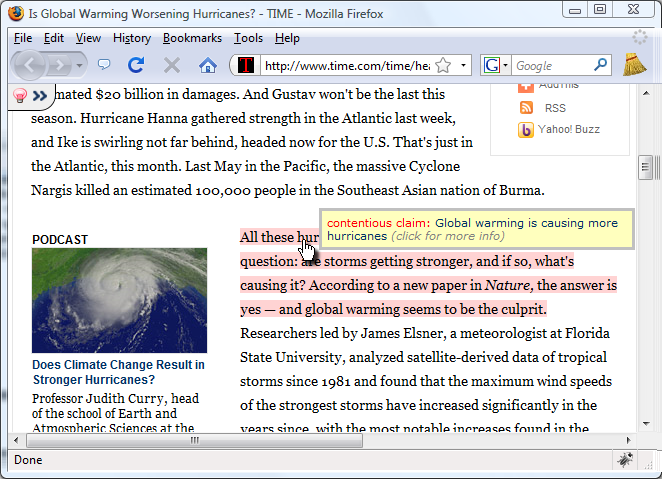
\includegraphics[width=8.5cm]{../screenshots/redhighlight.png}
	\caption{Think Link highlights the key claims made by a page. Red means the claim is contentious.}
	\label{highlight}
\end{figure}

\begin{figure}[ht]
	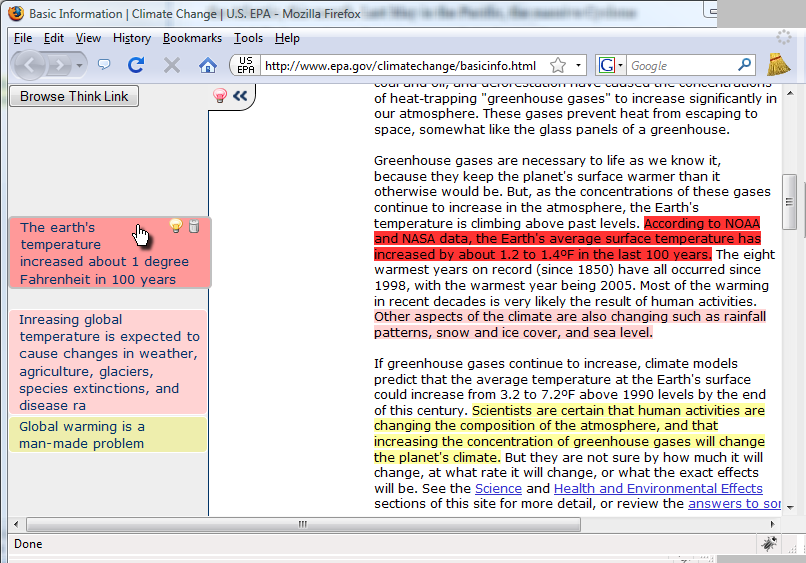
\includegraphics[width=8.5cm]{../screenshots/sidebar3.png}
	\caption{The margin shows a summary of the key claims made by the page}
	\label{margin}
\end{figure}

\begin{figure}[ht]
	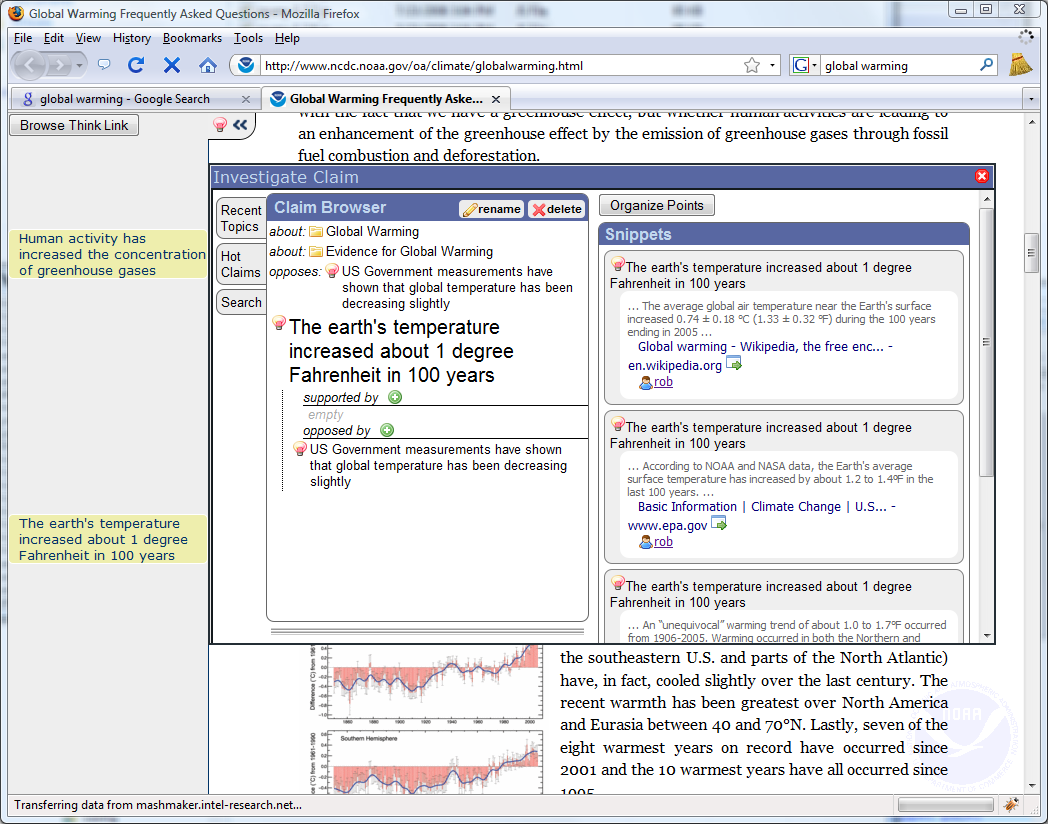
\includegraphics[width=8.5cm]{../screenshots/claim_popup.png}
	\caption{Click on a claim to see supporting or opposing evidence on other web pages}
	\label{claimview}
\end{figure}



\section{Introduction}

The web provides users with a huge number of pages they can read, but extracting useful factual information from these pages can be hard work. Not everything on the web is true. A web site may make claims that are contradicted by other web sites. If a user is to avoid incorrect claims then they will need to either stick to sources they can trust, or spend time looking for evidence on other web sites that supports or opposes what they have read. Similarly, not everything on the web is interesting. If a user wants to find interesting factual claims about a topic then they may have to waste time reading claims that they have either read elsewhere or do not find interesting in order to find the claims that interest them.

Several commentators have observed that there is a Media Echo Chamber effect~\cite{echochamber,echochamber2} in which news sources report claims that they have heard from other news sources, despite the fact that these claims may be misleading or untrue. If a user only reads news sources from a particular group then they may only be exposed to the views of that group and may not be aware that opposing views exist unless they actively seek them. Tim Berners Lee has expressed concern about the difficulty that people face discerning whether information on the web is true~\cite{bbcwebwarning}.

Part of the problem is that traditional web browsing tools require the user to browse by looking at pages, when it is often not the pages themselves that the user is interested in but the factual claims contained within them. While a web page will typically contain links to other pages, as chosen by the page author, it does not provide an easy way for a user to validate whether the claims made by a page are supported by evidence that may be available on other pages. Moreover the best arguments supporting or opposing a claim may be distributed across a large number of disconnected pages, making it difficult for a user to assemble an argument from the pages on the web. The web is structured around where knowledge is coming from (pages written by particular authors) rather than what knowledge is about (the ideas contained on the pages). While this makes it easier for add knowledge to the web, it makes it harder for users to extract factual claims from it.


\subsection{Browse the Web of Factual Claims}

We have created a tool called Think Link that connects pages on the web to the factual claims being made on those pages, and allows a user to quickly find snippets of text on other web pages that make supporting or opposing claims. We hope that this tool will make it easier for users to identify incorrect claims in documents they read, and to quickly identify the best arguments for and against claims that they may be interested in.

As a user browses a web page Think Link will highlight snippets of text that make factual claims (Figure~\ref{highlight}). If a factual claim is contentious (meaning that other pages make opposing claims) then the highlight will be red. More information about highlighted claims can be found by either mousing over one of them, or opening the Think Link margin (Figure~\ref{margin}).

These highlighted claims serve as entry points to a browsable graph of factual claims. Clicking on a claim will pop up a window that allows one to easily view the other claims that support or oppose the selected claim, and the snippets of text on the web that make these claims (Figure~\ref{claimview}).

For example, if a user browsed a web page that claimed ``Global Warming does not exist'', then the text snippet that made this claim would be highlighted in red, indicating the fact that there are web pages elsewhere that make opposing claims. If the user were to click on the highlighted snippet then an ``investigate claim'' window would appear. This window would show that the claim ``Global Warming does not exist'' is opposed by the claim ``There is strong evidence for global warming''. If the user navigated to this new claim then they could quickly see the best claims that support the existence of global warming, and would be able to see summaries of the best sources that supported these claims.

\subsection{Collaborating to connect claims}

Think Link shares a lot in common with Wikis like Wikipedia~\cite{wikipedia}. The claim graph is shared between all users and editable by anyone. Any user can identify a claim made on a web page by selecting the web snippet that makes this claim and clicking the ``new snippet'' button on the browser toolbar. Similarly, any user can establish new supporting and opposing relationships between claims by using drag and drop within the claim browser. One can think of Think Link as being rather like a Wiki in which all the content is clipped from existing sources and links are created from those sources back to the wiki.

Think Link uses collaborative filtering~\cite{collaborativefilter} to highlight the most interesting claims that support and oppose another claim, and the most interesting snippets that make a claim. If a user finds a snippet or claim interesting then they can mark it as such. When Think Link lists claims or snippets, it will show first those that the user marked as interesting, and order the rest according to the number of other users who marked them interesting.

\subsection{The Mental Model}

Think Link presents users with three kinds of object, each associated with a different family of icons:

\begin{itemize}
\item {\bf a claim} (
\includegraphics[width=0.3cm]{../images/lightbulb_off.png}) is a factual claim about the world that may be true or false. For example ``Global warming exists''. A claim may support or oppose other claims. Claims are written as raw English\footnote{though one can imagine supporting other languages in the future} text and are not understood logically by Think Link.
\item {\bf a snippet} (
\includegraphics[width=0.3cm]{../images/comment.png}) is a section of text on a particular web site that asserts or assumes the truth of a particular claim. Many snippets may assert the same claim and users are encouraged to re-use existing claims rather than creating new ones when creating new snippets.
\item {\bf a topic} (
\includegraphics[width=0.3cm]{../images/folder_grey.png}) is a thing that claims can be about. For example ``Global Warming'', or ``Computer Science''. A claim can have one or more topics that it is about, and a topic can have one or more more general topics. Topics are used both to organize, and to disambiguate claims. For example ``Bush'' can mean either ``George H W Bush'', ``George W Bush'', ``Vannevar Bush'', ``Kate Bush'', ``The Rock Band Bush'', or just ``A Bush''. Associating a claim with a topic allows one to write shorter claims without worrying about being ambiguous.
\end{itemize}

The three icons are used consistently when refering to these three object types. 
Yellow versions of these icons (
\includegraphics[width=0.3cm]{../images/lightbulb.png},
\includegraphics[width=0.3cm]{../images/folder.png},
\includegraphics[width=0.3cm]{../images/comment_yellow.png}) are used to identify claims, folders, or snippets that the user has marked as interesting.


\subsection{Why People Annotate}

Tools like Think Link rely on user contributions in order to be useful. If no users are identifying factual claims on pages then other people who browse such pages will not see any claims identified. Similarly, if no other users are connecting claims together, then users will not see any supporting or opposing claims when they click on a highlighted snippet.

Moreover, in order to become popular, a tool like Think Link needs to be useful even when very few people are using it. If a tool is only useful when it has a large community using it then it is unlikely that early adopters will stick with it enough for it to ever acquire a large community.

Our user study participants identified several reasons why they would want to mark up factual claims in documents they found. The most common reason people gave for identifying and organizing factual claims was if the person was writing an article or researching a topic and wanted to keep track of the information they had found. One user (who was an active blogger) also expressed an interest in finding and marking up instances of claims that he disagreed with, so that readers would see the arguments highlighted in red and be directed to the counter-arguments. The same user also expressed an interest in marking up claims in documents he had made in his own articles so that readers could quickly see the evidence he had found in support of his claims.

\studyresult{Quotes of users saying why they would use it}

\subsection{Contributions}

We believe that this work makes the following key contributions:

\begin{itemize}
\item We propose a new approach to browsing web pages that focusses on the factual claims made by these articles
\item We develop interaction techniques that make it easy for a user to browse the web through factual claims
\end{itemize}

\section{Interaction Techniques}

Users interact with Think Link in four key ways. Think Link will draw attention to interesting claims on pages that the user browses; it allows the user to identify new factual claims on pages they browse; it allows them to browse the graph of related claims and identify the strongest evidence supporting or opposing the claims they are looking at; and it allows them to organize the claim graph by making new connections between existing claims and topics.

\subsection{Identifying factual claims on a page}

When a user browses a web page, we want to make them aware of claims being made on the page that they might find interesting, or that other sources disagree with. Think Link draws attention to the factual claims that other users have identified on a web page by highlighting them (Figure~\ref{highlight}). Snippets are highlighted in red if they are contenious (other sources disagree with the claim), or yellow otherwise. The highlight colors are chosen such as to be pale enough to not impede reading, but dark enough to be noticeable. The colors are chosen to fit with people's normal associations with colors, where red is commonly associated with danger (e.g. a traffic light) and yellow is the standard color used for highlighter pens.

While a highlight lets the user know that a the snippet is making an interesting or contentious claim, the user may still wonder what claim the snippet has been identified as making. A snippet could be interpreted as asserting the truth of several claims. For example the phrase ``Alice and Bob live in Canada'' asserts both that Alice lives in Canada and that Bob lives in Canada. Similarly, a user may have eroneously marked a snippet as asserting a claim that it does not directly assert to be true. For example ``Alice and Bob live together''.

There are two ways that a user can identify the claims being made by the highlighted snippet; they can either hover their mose over a particular snippet to show information about that snippet (Figure~\ref{highlight}, or they can use the Think Link margin to show information about all snippets on the page (Figure~\ref{margin}).

The Think Link Margin is designed to mimick the traditional margin notes that readers often write on physical documents they are reading~\cite{marginalia}. A margin space is added to the left of the page containing a margin note for each snippet. Each margin note is aligned vertically with the claim it is about and contains the text of the claim. To emphasise the connection between a margin note and its associated snippet, a snippet is highlighted more strongly when the user mouses over the associated margin note (Figure~\ref{margin}). 

We found that when a participant sees a highlighted snippet, they will typically want to do one of four things: ignore it, remember it, delete it, or investigate it. If the user finds the snippet interesting and wants to use it later then they can bookmark it by clicking the bookmark icon that pops up when they mouse over the margin note. This will cause it to be displayed prominently in the claim browser (Section~\ref{browseclaims}). If the user believes the snippet to not be making the claim that it says it does or otherwise badly marked up then they can delete the snippet by clicking on the trash can icon on the margin note. If the user thinks the claim is interesting and wants to see how it relates to claims made by other snippets on the web then they can click on either the highlighted text or the margin note to open the claim browser (Section~\ref{browseclaims}).

A user can also use the margin to provide a quick overview of a document. They can scroll quickly through the document and look to see what key claims other users have marked in the margins. Several users remarked on how useful it was when reading a long document to be able to quickly scan through it and see what other users have thought were the most interesting points. \studyresult{put in some quotes}

\todo{sort out more consistent colors and icons between this view and the web view}
\todo{give the margin consistent colors with the highlight sections}
\todo{more nice zoomed-in screenshots showing the different interaction techniques}

\subsection{Identifying new factual claims}

\begin{figure}[t]
	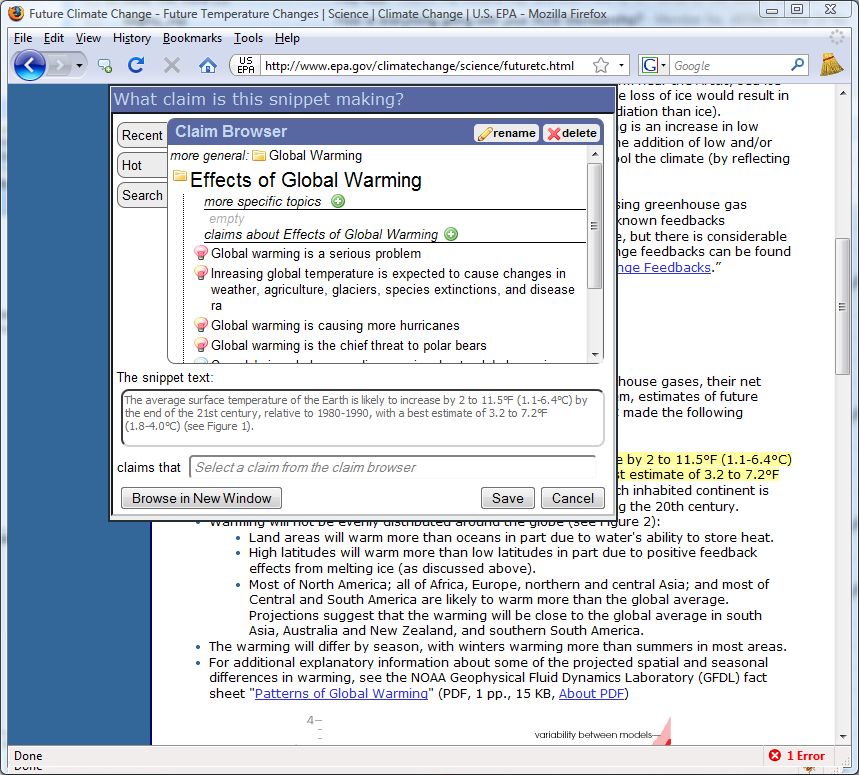
\includegraphics[width=8.5cm]{../screenshots/snipsave_full.png}
	\caption{The claim selection window allows one to identify the claim a snippet is making}
	\label{snipsavefull}
\end{figure}

\begin{figure}[t]
	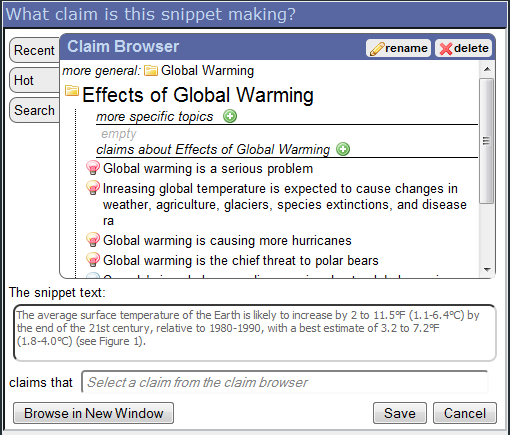
\includegraphics[width=8.5cm]{../screenshots/snipsave_crop.png}
	\caption{Close up view of the claim selection window}
	\label{snipsavecrop}
\end{figure}


If a user finds a snippet of text on a page that makes an interesting claim then they may want to enter it into Think Link. There are several reasons they may wish to do this. It may be that they find the snippet useful and may want to refer to it again in the future. It may be that they disagree with the claim, and want to alert other readers to the fact that there are opposing arguments, or it may be that they agree with the claim and want to provide easy access to evidence that backs it up. 

To create a new snippet, the user selects the text to be included and then either clicks on the ``new snippet'' button on the browser toolbar, or selects the ``new snippet'' option from the context menu that appears when they click the right mouse button. This is a similar approach to that taken clipping tools such as Google Notebook~\cite{googlenotebook}.

Once the user has identified the text in a snippet, they need to identify the claim that the snippet is making. To do this, Think Link presents the user with a ``claim selection'' window. This window contains a small version of the claim browser (Section~\ref{browseclaim}) that the user can use to select the claim that the snippet is making. At the bottom of the window, we show the phrase ``the snippet text {\it snippet} claims that {\it claim}''. We found that this helps users understand the nature of a claim and its relationship to a snippet (Section~\ref{study-claimmeaning}).

Since much of Think Link's utility comes from linking snippets together, it is important that to encourage users to reuse existing claims rather than creating new ones, and that when users do create new claims they connect them to existing claims and existing topics. Motivated by this, we designed the claim selection window to make it easier to pick out an existing claim than to create a new one. Moreover, one cannot create a new claim without connecting it to an existing topic or an existing claim. To create a new claim, one navigates to a topic that the claim is about, or a claim that the new claim supports or opposes, and then clicks on the (
\includegraphics[width=0.3cm]{../images/add.png}) button on the list that one wishes to add the new claim to. For example, if the new claim opposes an existing claim, then one clicks the (
\includegraphics[width=0.3cm]{../images/add.png}) button on the ``opposed by'' heading for the existing claim.

This is an intentionally different model to that used by ad-hoc tag-based~\cite{tags} systems such as Delicious~\cite{delicious} and Flickr~\cite{flickr}. This is because in bookmarking or image storing systems it is not so important that duplicates be avoided and that objects be well connected.

In earlier revisions of the interface it was very easy for users to quickly create new claim texts and awkward to find and reuse existing ones. This led users to create many claims that were essentially equivalent and reduced the utility of Think Link as a tool for connection snippets together (Section~\ref{study-reuse}). 

\todo{Make new snippet icon throb when something is selected}

\subsection{Browsing factual claims}
\label{browseclaim}

\begin{figure}[ht]
	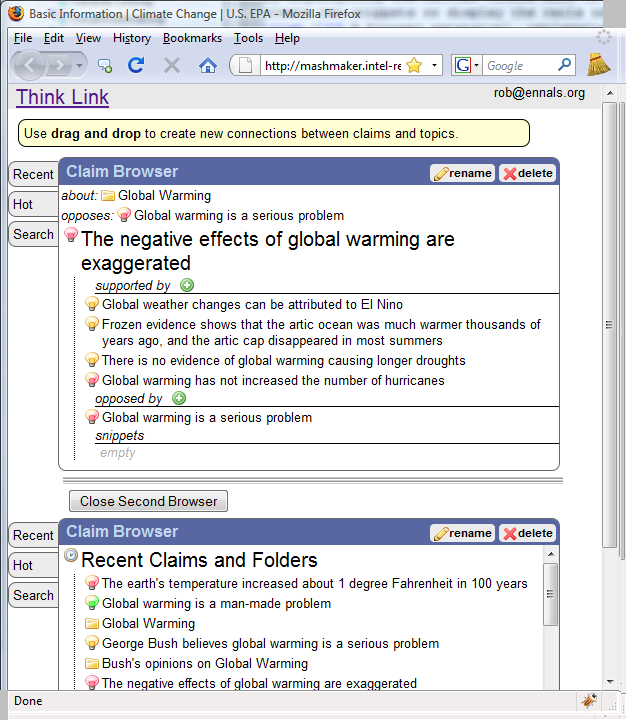
\includegraphics[width=8.5cm]{../screenshots/claimbrowse.png}
	\caption{The Claim Browser}
	\label{fig:claimbrowser}
\end{figure}

Our users expressed an interest in using snippets to help them construct arguments that support a claim they agree with, to show them the arguments for and against a claim that they are unsure about, to collect evidence about a topic they are interested in, to share information with friends, and to see arguments against claims that they encountered on the web. We constructed the ``claim browser'' interface to help users do these things (Figure~\ref{fig:claimbrowser}).

Claims and topics form a directed graph structure. A claim can have any number of claims that support or oppose it, and any number of claims that it supports or opposes.
A topic can have any number of more specific topics (e.g. ``US Election 2008'' is more specific than ``US Elections'') and any number of more general topics. A topic can also have any number of claims about that topic.

When designing an interface to this structure, we were faced with two opposing constraints. We needed to be able to clearly view a large number of claims and topics in a small screen space, and we needed an interface that made it clear that the data was a graph rather than a tree. Dynamically reorganizing graphs such as those used in Vizster~\cite{vizster} and Personal Brain~\cite{thebrain} made the graph structure very clear, but made it difficult to clearly view large numbers of claims. Tree-based outliners such as OmniOutliner~\cite{outliner} made it easy to view large numbers of related claims, but made it difficult to present an impression of the data being a graph rather than a tree.

\todo{This interface is actually closer to TheBrain than the text suggests}

After several iterations, we settled on an interface that is a dynamically reorganizing graph layed out like an outliner. Like other dynamically reorganizing graphs, the interface is arranged around the currently selected node, and when a new node is selected the interface animates to surround the newly selected node with objects to relate to it. Like an outliner, the nodes that relate to the selected node are listed vertically below the selected node, each on their own line. Our users commented that they found it quite intuitive to navigate through a graph of claims and topics in this way. \studyresult{quote}.

The placement of objects above and below is intended to emphasize the conventional structuring of an argument graph (Section~\ref{argumentgraph}), with topics going upwards and arguments for and against a claim going downwards. A user can navigate down to get to explore why a claim may or may not be true, or navigate up to find out about more general topics, or claims that the selected claim supports or opposes.

\todo{Have I seen an interface like this elsewhere? Did PARC have something like this?}

\todo{Is this interface a contribution in itself? Has an interface like this been presented before?}

Animation is used throughout the interface to give users a sense of where they are and how the current interface state related to previous states. When a new item is selected, it grows in size and moves to the center. Other items that were already on the screen move from their current locations to their new locations. Other objects appear and disapper by smoothly sliding into or out of view. We found that this animation helps users retain a sense of where they are with respect to what they were looking at previously and helps users avoid getting lost (Section~\ref{gettinglost}).

Users see a claim browser in three different places:
\begin{itemize}
\item {\bf The Main Organizer} shows two claim browsers, and allows users to use drag and drop to make new connections between claims in the two organizers. (Figure~\ref{fig:claimbrowser})
\item {\bf The Popup Browser} shows one claim browser in a reduced-size window and is used to quickly investigate a claim found on a web page. (Figure~\ref{claimview})
\item {\bf The Claim Selection Window} shows one claim browser, together with the text of a new snippet, and is used to identify the claim that a snippet is making. (Figure~\ref{snipsavefull}) 
\end{itemize}


\subsection{Organizing factual claims}

Much of the value of Think Link comes from the connections between claims. It is thus important that it be easy to establish new connections between claims and topics. 

Think Link uses the familiar drag and drop interface for establishing new connections. To establish a connection between two claims, one need simply drag one claim onto the other. In the full interface, one can open two browsers and drag points from one browser onto points on the other.

In our initial study, we found that many users did not realize that they could use drag and drop to create connections to existing claims. We rectify this, we added a notice at the top of the main organizer window (Figure~\ref{fig:claimbrowser}) telling users that they can use drag and drop.

We found that creating new connections between existing claims was one of the things that users found most difficult.

\todo{say more here}

\section{Discussion}

\subsection{Context of a Claim}

\subsection{How many claims to show}

\subsection{Beyond Claims}

\section{Implementation}

Think Link is implemented as three largely independent components:

\begin{itemize}
\item {\bf A server}, written using Ruby, PHP, and MySQL that maintains a graph of claims, topics, and snippets and provides an API that allows this data to be queried and modified
\item {\bf A web UI}, written using Ruby on Rails~\cite{rails} that provides a visual interface to the claim graph
\item {\bf A page enhancement script}, written in Javascript, that augments the page it is run on by highlighting the factual claims made on the page. This script also provides the ability to create new snippets or display the rails interface to investigate a particular claim.
\item {\bf A browser extension}, implemented for Firefox~\cite{firefoxextension}, that inserts the page enhancement script into all pages the user browses to, and provides toolbar and context-menu shortcuts to the ``new snippet'' feature of the page enhancement script.
\end{itemize}

These components are largely independent. One could use the javascript script on a web page without using the firefox extension, by either manually including it on the page (e.g. to enhance your own blog) or by adding it using a proxy. Since the server API is public, one could write alternative tools that mark up web pages in different ways, or use the claim graph for different purposes.

The source code to Think Link is publicly available under the Apache license at the following URL:

{\b url removed for blind submission}

We expect to have a public deployment available by the time of publication.

We use icons from the free FamFamFam Silk~\cite{silkicons} collection.



\section{Investigative Study}

We performed two ``think aloud'' studies to guide and evaluate the development of Think Link. The aim of the first study was to see how users normally browse the web and to see how they might try to use an initial prototype of Think Link to help them. 

\subsection{Protocol for the First Study}

We recruited 12 paid participants. Five were female, seven were male. Their ages ranged from high school age to retired. Our intention was to recruit users who were not experts, but who regularly used the internet to find information. We recruited participants using a posting to the Craigslist~\cite{craigslist} classified adverts site. In our advert, we expressed an interest in people who use the internet to gather knowledge, rather than just for tasks such as email or shopping. We filtered participants based on their short answers to questions about how they found, organized, and shared information on the web. 

\subsection{Study Protocol}

Study sessions took approximately 45 minutes. Participants were seated at a single-screen workstation with the Firefox browser, augmented with the Think Link plugin. We first demonstrated Think Link's interface, and then asked them to perform two tasks. In the first task, we asked them to use Think Link to gather information about a political topic that was of interest to them and currently in the news. For the second task, we asked them to browse the web in a way that would typically do so at home or at work, and see if they could use Think Link to help them do so.

In the second task, we wanted to leave users relatively unconstrained so that we could see how users might try to use a tool like this during their normal browsing, rather than how well they could accomplish a pre-set task that they might never attempt in normal life. For the first task, we constrained the task to an a topic for which we had already marked up a number of claims, to increase the likelyhood that users would encounter existing claims.


\subsection{Findings}

All the participants were able to create new snippets. Participants had little difficulty identifying interesting claims being made by web pages, selecting appropriate sections of text, and either picking existing claims that were appropriate, or writing appropriate new claims. Most ($9/12$) stated that they found it easy to create new snippets and associate them with claims.

In the initial interface, snippets were only highlighted when the margin was open. This confused some participants ($5/12$) who were surprised to not see their snippets highlighted when they created them. This led us to change the interface so that snippets were always highlighted.

In the initial interface, the button to open the margin was on the toolbar, next to the ``new snippet'' button, rather than 

Two participants initially had dificulty summarising text with a claim that the text was actually making, rather than an claim it was associated with.

Many ($7/12$) participants also expressed a desire to organize snippets and claims during their session. Of these seven, we noticed that four would alternate between creating new snippets and organizing their claims in the claim browser (Section~\ref{claimbrowser}). With each new claim, users would create relationships between existing claims.




\subsection{The Prototype Interface}

Participants were shown an earlier interface than that described in Section~\ref{interface}. 

\begin{figure}[ht]
	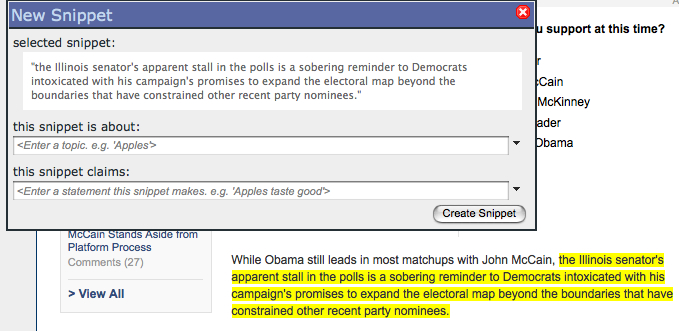
\includegraphics[scale=0.35]{../screenshots/snippetdialog_sm.jpg}
	\caption{First Prototype Snippet Creation Dialog}
	\label{oldsnippetbox}
\end{figure}


\subsection{Successes}

All the participants were able to create new snippets, succeeding in identifying appropriate sections of text that should be marked, and picking out either an appropriate existing claim, or creating a new claims that accurately summarized the snippet. Two participants initially had difficulty in correctly summarizing text with a claim that the text was actually making, but they eventually got used to it.

Many ($7/12$) participants also expressed a desire to organize snippets and claims during their session. Of these seven, we noticed that four would alternate between creating new snippets and organizing their claims in the claim browser (Section~\ref{claimbrowser}). With each new claim, users would create relationships between existing claims.

Most ($10/12$) either reused a topic that they had created themselves or that we had previously created. While the level of social activity was undoubtedly limited by the relatively small number of claims available in our database and the wide range of topics participants read about, three of the six people who browsed points in the 

\subsection{Observations Motivating Design Changes}


Many ($7/12$) participants also expressed the desire to organize snippets and points during their session. Of these seven, we noticed that four were alternating between creating snippets from new articles and organizing points in their {\it Recent Activity}: with each new snippet, users were creating relationships between points. When browsing web content about a particular topic or issue, most participants ($10/12$) either reused a topic that they created during their session or that someone else had created previously. Half of those ten used a topic that they {\it hadn't} created, demonstrating the ease of collaboration in our application. Both these organizational activities support connections inside the web of ideas. While the level of social activity was undoubtedly limited by the relatively small number of points (about $400$), three of the six people who browsed points in the main web interface looked at points created by other users. Two of the later study participants viewed someone else's point and either read the snippet text or viewed the originating document. As the number of points and topics increases, we expect to see more social behavior like this.



\subsection{Browsing Claims}

\subsection{Creating Snippets}


\section{Evaluation Study}

The purpose of the second study was to evaluate whether the interface changes we had made in reaction to the first study had made the tool usable. 

\subsection{Recruitment}

We recruited 6 paid participants. Four were female and two were male. Although we recruited participants using the same advert as the first study, the timing of our second advert around the beginning of the semester meant that five of the participants were students. Since the second group was different demographically to the first group, it is not possible to make a direct comparison between their behaviours. However we were still able to make interesting observations about how users used the new interface.

\subsection{Study Protocol}

For the second study, we changed the task to focus on how easy users found it to use the interface, rather than on how they might apply it to their normal browsing. We told users nothing about how to use the tool. Instead, we just gave them a brief introduction to what our tool was for, and then asked them to attempt two tasks. The first task was to look at a selection of web pages that already had highlights and tell them to explore the interface. The second task was to identify claims on a page that had not been marked up and connect them appropriately to existing claims.



\section{Related Work}

\subsection{Wikis}

\subsection{Web Annotation}

\subsection{Sensemaking}

\cite{scenthighlights}\cite{scenttrails}

\subsection{Argumentation Theory}

The 
\cite{Korb97acognitive}
\cite{toulmin}
\cite{carneades}
\cite{conceptmap}
\cite{argmas}

Memex
Vannevar 
Bush's vision of Memex. Bush popularized the idea that 
people can collaboratively organize and share knowledge: 
``Wholly new forms of encyclopedias will appear, ready-made 
with a mesh of associative trails running through them...'' 
[5]. In many ways the vision has come to pass with large 
amounts of hyper-linked information in the World Wide 
Web, digital libraries, and online encyclopedias. However, 
researchers continue to point out that people, especially 
those lacking domain expertise, struggle to navigate infor- 
mation spaces. 


\subsection{Identifying Ideas on the Web}

\cite{quotations}, \cite{quotationdl} Overall aim is to identify and connect ideas. Do quotation matching as a partial solution.

\cite{scenthighlights}

\cite{ideanavigation}, \cite{citesense}


\subsection{Web Annotation Systems}

\cite{personalweb}

Diigo lets you save, import, tag, highlight, mark up and share Web pages
	select content on webpage
	share bookmarked content; bookmark url and see what people have tagged on that page
	search over collection of selected content
	tag selected content; social tagging
	see friends activity; more social behavior than necessary (eg. msging)
	meet people ``like'' me?
Stickis
Fleck
Shiftspace
SharedCopy
JKN
MyStickies
DrawHere

- UIs for highlighting
- wikipedia highlighting not trustworthy stuff

\subsection{Web Clippings}

Google Notebook
Trailfire
Zotero~\cite{zotero} is a citation mangament tool. Find and organise sources, while recording author, date etc by understanding pages. Can add notes to sources.
Scrapbook~\cite{scrapbook}

\subsection{Semantic Linking}

\subsection{Social Bookmarking}

Shadows

\subsection{User Contributed Links}

Memex allowed users to describe their own paths between pages, rather than requiring the page authors to modify them.

Everything2 creates soft-links between documents based on the browsing patterns of users.

ENQUIRE contains bi-directional links that show who links to a document. TrackBack does the same.

\subsection{Automated Reasoning}

Case-Based reasoning
Sensemaking

\subsection{Argumentation Graphs}
Argumentation graphs express positions and arguments in a formal graph model as nodes and edges, respectively, and are typically used to make a decision or draw a conclusion about some issue. One example implementation is the {\it Zeno} argumentation framework~\cite{zeno}, designed for collaborative use in mediation systems to debate the quality of alternative solutions for a problem. In their object model of argumentation elements, based on Rittel's IBIS model~\cite{ibis}, example nodes include pro/con arguments, positions, preferences, comments, and decisions. Importantly, arguments are connected via {\it consequent} and {\it antecedent} edges, which are used to inform {\it choices}. The decision-making power of the argumentation graph follows from the traversal of argument relationships to enhance the depth and breadth of understanding about an issue. Our application similarly links claims as {\it supporting} and {\it opposing} other claims to allow users to develop a cohesive understanding of arguments.

Traditional argumentation graphs are designed to solve a specific, isolated issue. Our application supports an ever-expanding set of topics, and arguments can form links between multiple topics. Users can consult the web of ideas directly to form an opinion about a particular issue, but they can also browse for new issues to explore. Opinions or decisions in our model don't have to be static: as the topic is expanded with more supporting and opposing evidence, users may alter previous viewpoints. Another advantage of our model is that the ability to explore claims' source-document evidence is built right into the navigation. Looking at an argument shows both its related argument as well as its supporting {\it snippets}, allowing the user to explore the evidence for himself. 



\section{Observations Informing Design}


\subsection{Recruitment}
Our user study participants were selected from a pool of respondents to a Craigslist posting for people who use the internet as one of their primary sources of information, regularly gather and share this information, and are interested in a new application to facilitate that process. We chose participants based on their responses to the following questions:
\begin{enumerate}
	\item What topics or types of information do you usually look for on the internet?
	\item How do usually go about finding information? (e.g. google, digg, friends, etc)
	\item How do you organize the information you find? (e.g. text file, paper, wiki, etc)
	\item How do you share information with others? (e.g. blog posts, comments, email, facebook, etc)
\end{enumerate}
We preferred individuals who search the internet for research and reading news rather than online shopping, as well as those interested in social and collaborative web activities like social networking web sites.  We were also interested in those who seemed to express a need for our application: people who copy-and-paste text from web pages into word processing documents, or who regularly email web page addresses to friends. Twelve people were selected to participate in this study.

\subsection{Study Environment}
Each study session lasted between thirty to forty-five minutes, with the participant sitting at a desktop computer with the Firefox browser running the application plugin. The session was a Think-Aloud study in which the participant verbally describes his/her thoughts throughout the duration of the study. A video camera captured the audio/video and was focused on the monitor screen. Before the session began, we briefly demonstrated the features of the application: how to (1) select snippets, (2) write a snippet topic and point, (3) relate points, (4) show/hide the margin, and (5) browse recent activity.

\subsection{Study Tasks}
The study consisted of two tasks to collect snippets, each lasting ten to fifteen minutes. During both tasks, we asked participants to browse the web as they normally would. In the first task, the participant browses the web about a topic or issue of their choice from the domain of politics. The collection of snippets should help the participant either argue or form an opinion/perspective about the topic, and should be thought of being used to help him/her explain or discuss the topic with a friend.  We constrained the first task to politics to increase the likelihood that the study participants would encounter similar issues and news stories.

For the second task, the participant was allowed to browse for any topic of their choosing. While the likelihood of topic overlap across participants was much lower, we were able to observe their behavior when searching for information in which each person had genuine interest.

At the conclusion of the session, we asked the participant if the application is something that would be likely to use, and for what purposes they would find it most useful. Any confusing features or experiences were also noted.

\subsection{Observations and Discussion}
% observed good and bad things
% good things validate the application's usefulness and applicability
% snippet selection super easy
% organization part a little lacking
% bad things we have ideas how to fix: UI redesign and smaller second study
% not as much social stuff going on, but limited stuff in DB for overlap to happen (more social stuff towards end of study)


{\it Note:} The first four study participants used a version of the web interface in which point relationships were constructed by navigating to one point page, searching for or typing the text of another point, and then expressing a directional relationship via a drop-down menu. We saw that participants found this process cumbersome and were less inclined to do it. Three of the four noted their confusion by the directional terms {\it supports} versus {\it is supported by}, and expressed a need for a more visual technique for constructing relationships. We modified the interface to allow users to drag and drop points on top of one another, with just the choice of {\it supports} and {\it opposes}. Half of the four participants were also confused by the Gmail-like labels alongside listed points that specified the topics each point belongs to.  The interface was modified to show topics listed with their related points beneath them. The remainder of the study used the modified interface. 

%hopefully more social uses when have more stuff in database

\subsubsection{Validating Observations?}
In general, the user study demonstrated that our application successfully allows people to associate portions of web content with ideas, and to organize and share those ideas. All the study participants were able to create new snippets, and only a couple ($2/12$) had initial difficulty in correctly summarizing snippet text into a point. Most participants ($10/12$) were interested in viewing the margin as they were creating new snippets. These observations demonstrate that snippet creation is easy for most users.

Many ($7/12$) participants also expressed the desire to organize snippets and points during their session. Of these seven, we noticed that four were alternating between creating snippets from new articles and organizing points in their {\it Recent Activity}: with each new snippet, users were creating relationships between points. When browsing web content about a particular topic or issue, most participants ($10/12$) either reused a topic that they created during their session or that someone else had created previously. Half of those ten used a topic that they {\it hadn't} created, demonstrating the ease of collaboration in our application. Both these organizational activities support connections inside the web of ideas. While the level of social activity was undoubtedly limited by the relatively small number of points (about $400$), three of the six people who browsed points in the main web interface looked at points created by other users. Two of the later study participants viewed someone else's point and either read the snippet text or viewed the originating document. As the number of points and topics increases, we expect to see more social behavior like this.

% easy to create snippets and view margin
% participants expressed desire to organize
% saw social activity and browsing
% (see more in usage types)
% not as much social stuff going on, but limited stuff in DB for overlap to happen (more social stuff towards end of study)

\subsubsection{Suggested Usage}
Many of the study participants who said they would our application suggested uses that match those described in our motivation, validating our prescribed use cases.  We identified the following use types, based on participant responses. Note that these many people suggested multiple use types.

\textbf{Blogging and writing:} Snippet collections are useful when gathering evidence and supporting material for a blog entry, report, or any kind of written composition. This use case necessitates the ability to organize, order, and rearrange snippets to best tell a story, generate a persuasive argument, or facilitate forming an opinion.

\textbf{Self-Bookmarking:} Creating snippets can be a means of bookmarking web page content that a user will return to for his/her own needs. These bookmarks are more specific than the web address of the page itself, and was suggested by users who currently find themselves cutting and pasting web content into a word processing file. This use case is more for retaining factual information than constructing an argument, although the information could also be used for the writing usage type.

\textbf{Social:} Sharing snippets with friends or targeted interest groups allows users to see what web content is interesting to people they follow. This use case is applicable both to those who wish to collaboratively generate a collection of information and to those who like sharing and browsing information from friends.

% Not for everyone! 3/12 people used it "incorrectly"
Several of the study participants suggested specific use cases that mirror our initial motivation for the application. One example was a user who would use snippets to as supporting evidence for asserting the incorrectness of someone else's claim on a web forum, as simple comments are not as effective. Our application, however, is not for everyone. Three of the twelve user study participants used (or wanted to use) our application ``incorrectly,'' e.g. to compare airline flight prices.


\section{Interaction Techniques}

\subsection{Features}
descriptions and screenshots: margin, snippet creation, relationship creation, web UI, point browser
\begin{figure}[ht]
	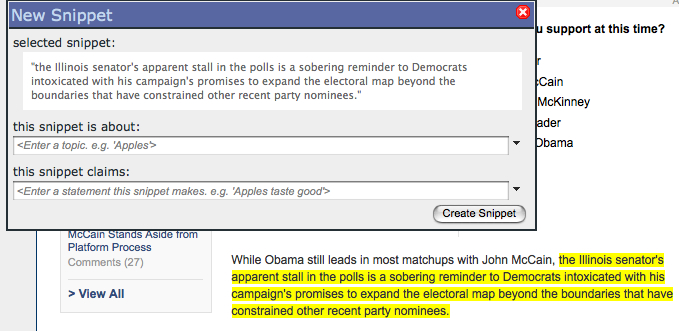
\includegraphics[scale=0.35]{../screenshots/snippetdialog_sm.jpg}
	\caption{Snippet creation dialog}
	\label{snippetdialog}
\end{figure}

\begin{figure}[ht]
	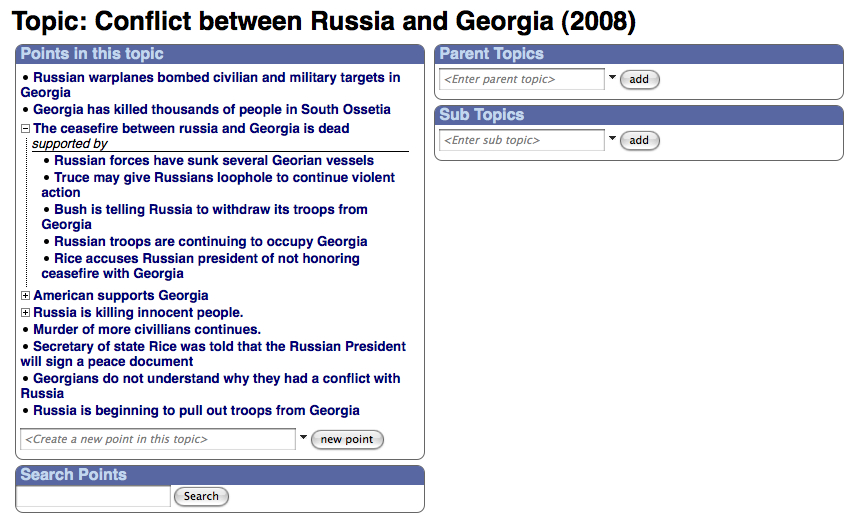
\includegraphics[scale=0.3]{../screenshots/topicpage_sm.jpg}
	\caption{Example topic page}
	\label{topicpage}
\end{figure}

\subsection{Implementation Decisions}

\idea{Wiki model not appropriate for points since want to manipulate several points at once}
\idea{Need to visualize relationships in web of ideas}


% \section{Creating Knowledge}
% 
% \section{Sharing Knowledge}
% 
% Why do users g
% 
% \section{Using Knowledge}
% 
% \section{Querying Data}


\section{Preliminary User Feedback}


1.5pp: recruitment, environment, tasks, observations, smaller study

\subsubsection{User Interface Redesign}
The first user study demonstrated a few flaws in the application's user interface. These problems can be generalized as:
\begin{itemize}
	\item \textbf{People need to easily visualize the the hierarchy of points, topics, and relationships.} A significant portion of the participants ($5/12$) explicitly expressed confusion about not being able to view the entire hierarchy of topics and points, and felt lost when looking at the individual point or topic pages. In this view, each point and topic is visually separated from its related points and topics, and thus users did not understand the significance of these individual pages. Viewing related points as lists of {\it child} and {\it parent} points was confusing to three of the eight people who used the second version of the UI. This ``flattened'' perspective also makes it difficult to relate several points to another. Most of the users who linked points together ($5/7$) did not recognize the need to first create an intermediate point and then relate other points to that new point. An easier model for grouping and associating objects together is necessary.
	\item \textbf{People need better organization capabilities at snippet creation time.} Only a few ($3/12$) users went back to their {\it Recent Activity} to create additional topics when organizing, which suggests that a majority of users prefer to place snippets within topics when they are first created. However, if users are only allowed to assign a snippet to one topic without context of a topic hierarchy, they may create a very specific topic that is unlikely to be used by another person. We observed this behavior with two participants who both created snippets regarding a politician's controversial affair, but whose snippets did not belong to related topics. Several participants ($4/12$) remarked that they were unsure how broad a topic should be. By allowing users to create and traverse the topic hierarchy, they would be able to more easily organize and specify new topics when creating a snippet.
\end{itemize}

Our solution to these problems was to redesign the user interface to resemble the traditional file browser. The left-hand side shows the expandable/collapsable hierarchy and shortcut paths, while the right-hand side shows a content preview of the selected item from the left. For example, when a point is selected, the preview shows its snippets and related points. Snippet creation will resemble a \texttt{save as...} dialog where users can easily traverse the topic/point hierarchy, and create new topics inside existing ones as deemed necessary.
This solution was implemented and used in a smaller user study. See section \ref{secondstudy}.

\idea{remove confusion about ``where i am'' with fisheye view of current claim}

\subsubsection{Second User Study}
\label{secondstudy}
There were six study participants who used the redesigned web interface.
\studyresult{we solved organization difficulties with this redesign}


%\section{Evaluation}

\section{Future Work}
1p: social queries, NLP stuff

\section{Conclusions}
$1/2$p


\bibliographystyle{abbrv}
\bibliography{biblio}

\end{document}
